\newpage
\subsection{Rancangan Detail Komponen}
\label{subsection:detail-komponen}

Berdasarkan rancangan struktural yang sudah dijelaskan pada bagian \ref{subsection:rancangan-struktural}, sistem akan diimplementasikan sebagai kumpulan komponen. Masing-masing komponen tersebut memiliki peran dan tanggung jawab yang berbeda dalam sistem eksperimen. Pada bagian ini, akan dijelaskan lebih lanjut mengenai rancangan detail dari masing-masing komponen tersebut.

\subsection{Rancangan Detail Node}
\label{subsection:detail-node}

Seperti yang sudah dijelaskan pada bagian \ref{sec:rancangan-struktural}, \textit{Node} merupakan satuan fungsional utama yang berperan sebagai entitas dalam sistem \textit{database} terdistribusi yang dikembangkan.

Struktur \textit{Node} terdiri dari:

\begin{enumerate}
    \item Subsistem penyimpanan: Subsistem ini bertanggung jawab untuk fungsionalitas \textit{key-value store} dalam sebuah \textit{Node}. Detail dari subsistem penyimpanan akan dijelaskan pada bagian \ref{subsection:detail-subsistem-penyimpanan}.
    \item Subsistem kontrol: Subsistem ini bertanggung jawab mengelola transaksi dan konsistensi antar-\textit{Node}. Detail dari subsistem kontrol akan dijelaskan pada bagian \ref{subsection:detail-subsistem-kontrol}.
    \item Komponen HTTP \textit{server}: Komponen ini berperan sebagai antarmuka komunikasi antara \textit{client} dan \textit{Node}. Detail dari komponen HTTP \textit{server} akan dijelaskan pada bagian \ref{subsection:detail-komponen-HTTP-server}.
    \item Komponen komunikasi antar-\textit{Node}: Komponen ini berfungsi untuk mengelola komunikasi antar-\textit{Node} dalam sistem terdistribusi. Detail dari komponen komunikasi antar-\textit{Node} akan dijelaskan pada bagian \ref{subsection:detail-subsistem-komunikasi-antar-node}.
\end{enumerate}

Ilustrasi struktur \textit{Node} dapat dilihat pada gambar \ref{fig:node-structure}.

% _TODO: Change image
\begin{figure}[ht]
    \centering
    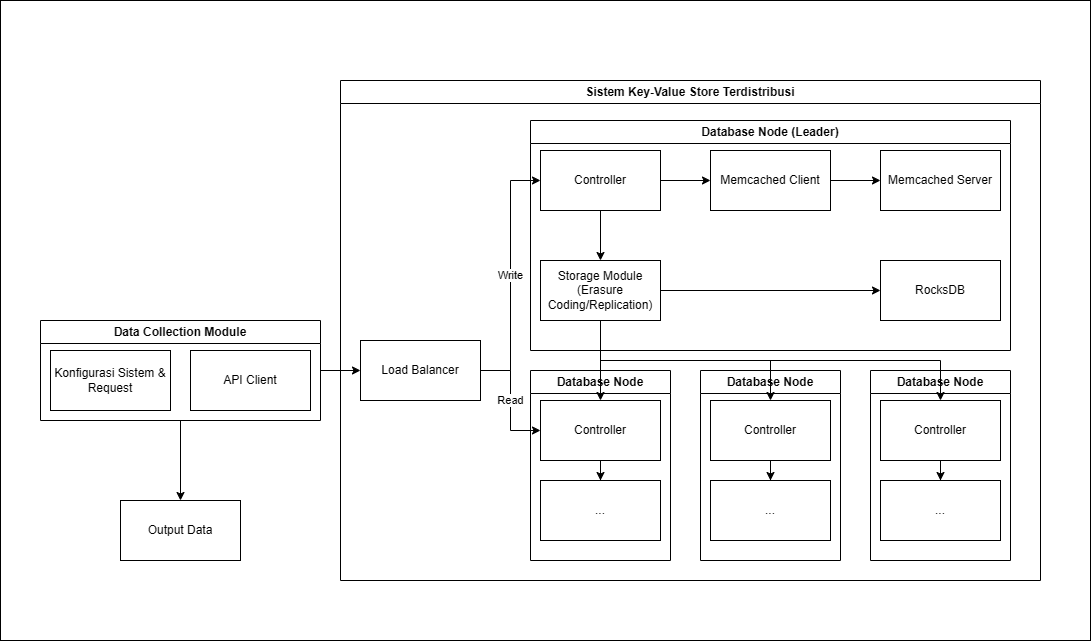
\includegraphics[width=0.95\textwidth]{resources/chapter-3/general-architecture.png}
    \caption{Struktur Node}
    \label{fig:node-structure}
\end{figure}
\subsubsection{Rancangan Detail Subsistem Penyimpanan}
\label{subsubsection:detail-subsistem-penyimpanan}

Subsistem penyimpanan adalah subsistem yang bertanggung jawab untuk fungsionalitas \textit{key-value store} dalam sebuah \textit{Node}. Subsistem ini akan terdiri atas komponen \textit{in-memory store}, \textit{persistent store}, \textit{transaction log}. Subsistem ini juga mengkonfigurasi \textit{Node} untuk menggunakan replikasi atau \textit{erasure coding}.

Mengikuti solusi yang sudah dipilih pada bagian \ref{sec:alternatif-solusi}, subsistem penyimpanan bersifat modular dengan Memcached sebagai \textit{in-memory key-value store} dan RocksDB sebagai \textit{persistent storage}. Memcached memiliki struktur \textit{server} dan \textit{client} sehingga subsistem ini berisi \textit{client} Memcached untuk berkomunikasi dengan \textit{server}. Pada rancangannya, dalam satu perangkat akan dijalankan satu \textit{server} Memcached untuk tiap \textit{Node} yang ada. Sementara itu, RocksDB dapat dijalankan pada tiap node tanpa memerlukan \textit{server}.

Ilustrasi struktur subsistem penyimpanan dapat dilihat pada gambar \ref{fig:storage-subsystem-structure}.

% _TODO: Change image
\begin{figure}[ht]
    \centering
    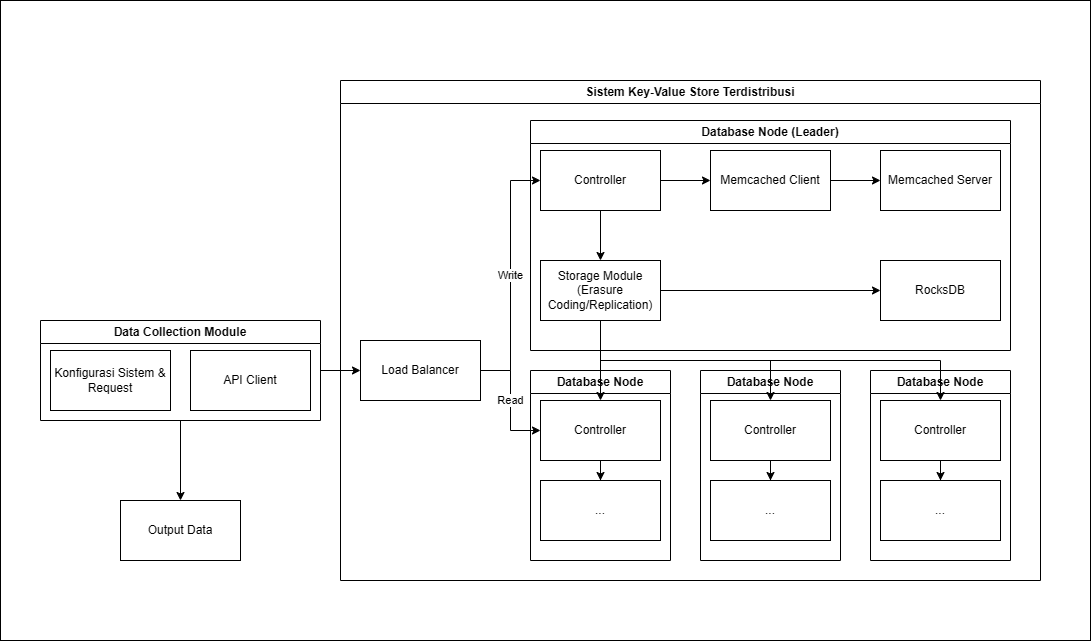
\includegraphics[width=0.95\textwidth]{resources/chapter-3/general-architecture.png}
    \caption{Struktur Subsistem Penyimpanan}
    \label{fig:storage-subsystem-structure}
\end{figure}

\subsubsection{Rancangan Detail Subsistem Kontrol}
\label{subsubsection:detail-subsistem-kontrol}
\subsubsection{Rancangan Detail Komponen HTTP Server}
\label{subsubsection:detail-komponen-HTTP-server}

Komponen HTTP \textit{server} berfungsi sebagai antarmuka komunikasi antara \textit{client} dan \textit{Node}. Komponen ini bertanggung jawab untuk menerima dan memproses permintaan dari \textit{client}, serta mengirimkan respons yang sesuai.

Ilustrasi struktur komponen HTTP \textit{server} dapat dilihat pada gambar \ref{fig:http-server-structure}.

% _TODO: Change image
\begin{figure}[ht]
    \centering
    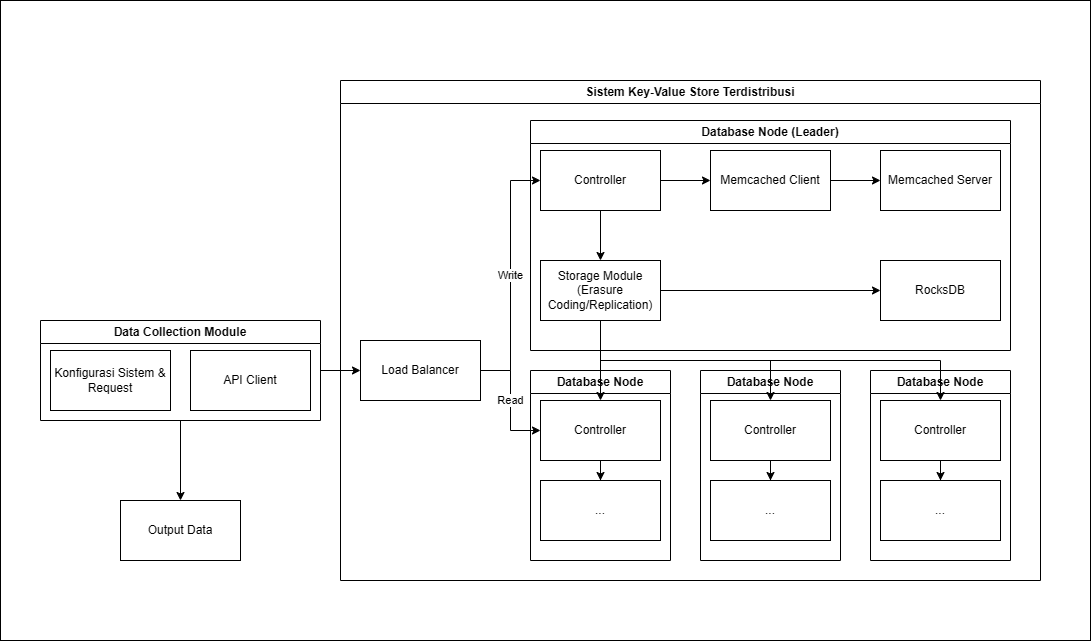
\includegraphics[width=0.95\textwidth]{resources/chapter-3/general-architecture.png}
    \caption{Struktur Komponen HTTP Server}
    \label{fig:http-server-structure}
\end{figure}

\subsubsection{Rancangan Detail Komponen Komunikasi Antar-Node}
\label{subsubsection:detail-subsistem-komunikasi-antar-node}

Komponen komunikasi antar-\textit{Node} bertanggung jawab untuk mengelola komunikasi antar-\textit{Node} dalam sistem terdistribusi. Komponen ini akan menggunakan protokol komunikasi yang sesuai untuk memastikan bahwa data dapat dikirim dan diterima.

Ilustrasi struktur komponen komunikasi antar-\textit{Node} dapat dilihat pada gambar \ref{fig:node-communication-structure}.

% _TODO: Change image
\begin{figure}[ht]
    \centering
    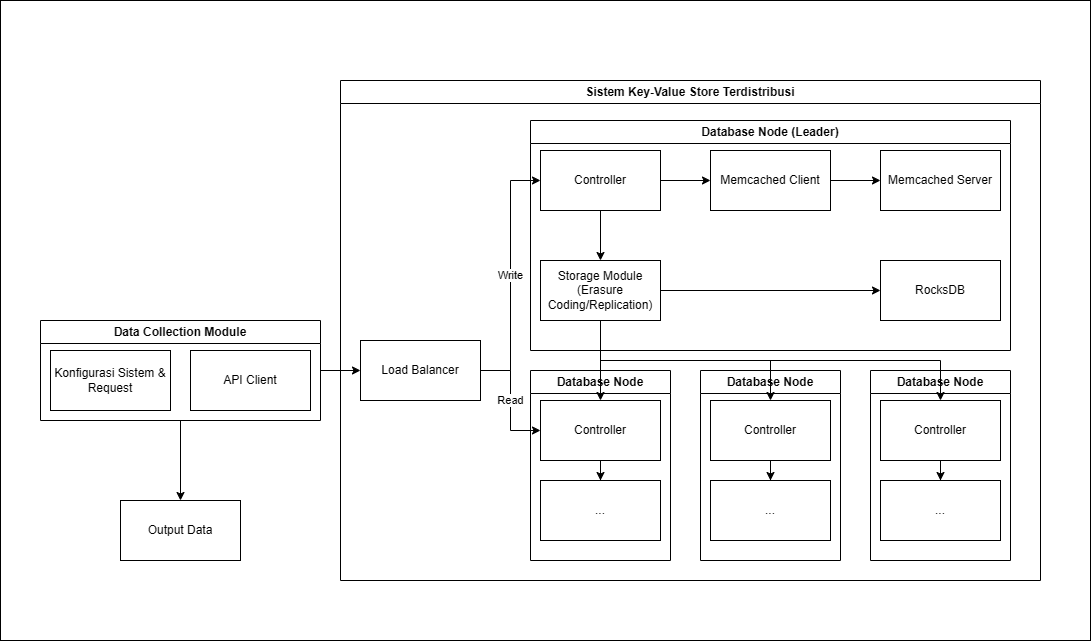
\includegraphics[width=0.95\textwidth]{resources/chapter-3/general-architecture.png}
    \caption{Struktur Komponen Komunikasi Antar-Node}
    \label{fig:node-communication-structure}
\end{figure}
\subsection{Rancangan Detail Data Collector}
\label{subsection:detail-data-collector}

Data Collector adalah komponen yang bertanggung jawab untuk mengumpulkan data dari sistem dan menyimpannya dalam format yang sesuai untuk analisis lebih lanjut. Komponen ini akan mengumpulkan data dari berbagai sumber, termasuk log sistem, metrik kinerja, dan informasi lainnya yang relevan.
Data Collector juga akan menyediakan antarmuka untuk mengakses data yang telah dikumpulkan, sehingga memudahkan pengguna untuk melakukan analisis dan visualisasi data.

Struktur \textit{Data Collector} terdiri dari:

\begin{enumerate}
    \item Komponen testing: Komponen ini bertanggung jawab untuk melakukan \textit{request} dan transaksi pada sistem.
    \item Komponen \textit{logging} dan \textit{tracing}: Komponen ini mengelola pencatatan dan pelacakan operasi yang dilakukan oleh sistem secara keseluruhan.
    \item Komponen \textit{reporting}: Komponen ini bertanggung jawab untuk mengumpulkan dan menyajikan hasil eksperimen dalam bentuk laporan.
\end{enumerate}

Ilustrasi struktur Data Collector dapat dilihat pada gambar \ref{fig:data-collector-structure}.

% _TODO: Change image
\begin{figure}[ht]
    \centering
    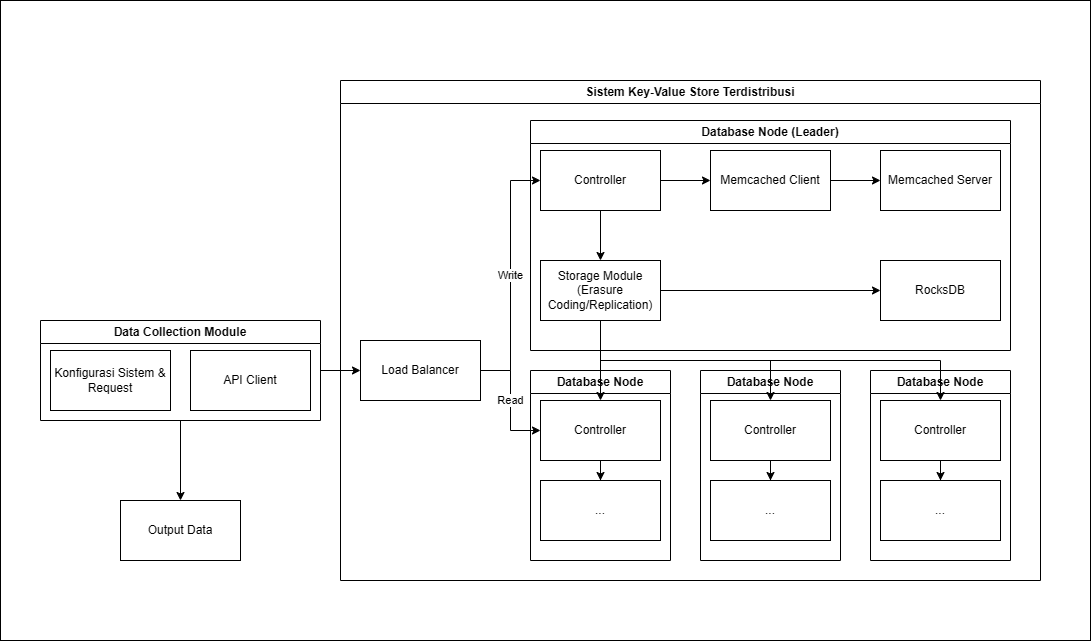
\includegraphics[width=0.95\textwidth]{resources/chapter-3/general-architecture.png}
    \caption{Struktur Data Collector}
    \label{fig:data-collector-structure}
\end{figure}
\subsubsection{Rancangan Detail Komponen Testing}
\label{subsubsection:detail-data-collector}

Komponen \textit{testing} bertanggung jawab untuk melakukan pengujian terhadap sistem yang telah dibangun. Pengujian ini dilakukan untuk memastikan bahwa sistem berfungsi sesuai dengan spesifikasi yang telah ditentukan. Komponen ini juga bertanggung jawab untuk menghasilkan data yang kemudian dimasukkan ke komponen \textit{reporting} untuk visualisasi dan analisis.

Ilustrasi struktur komponen \textit{testing} dapat dilihat pada gambar \ref{fig:testing-structure}.

% _TODO: Change image
\begin{figure}[ht]
    \centering
    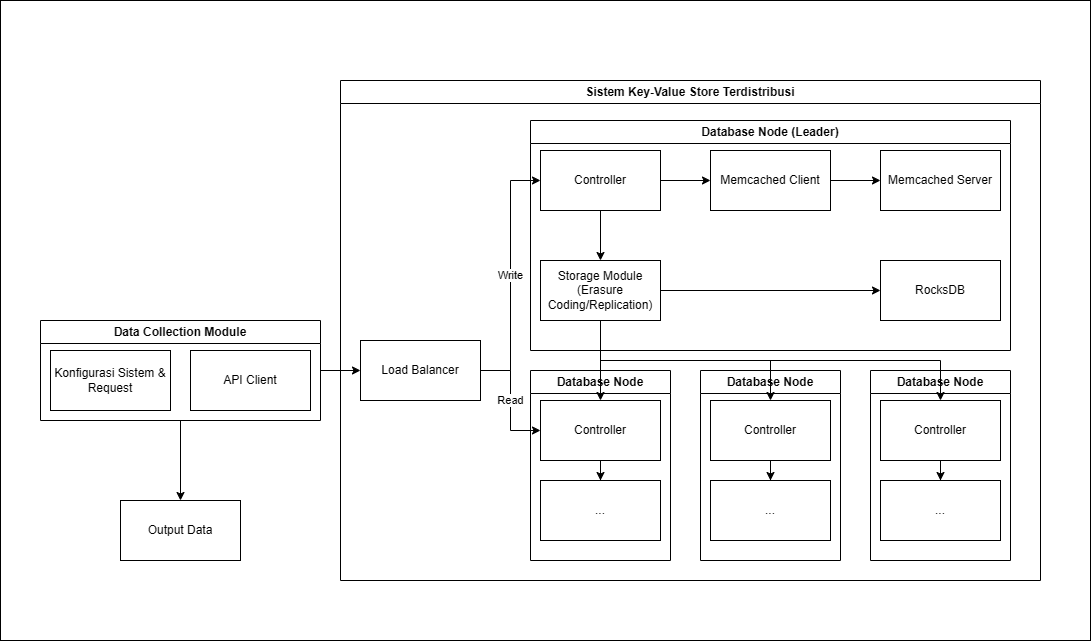
\includegraphics[width=0.95\textwidth]{resources/chapter-3/general-architecture.png}
    \caption{Struktur Komponen Testing}
    \label{fig:testing-structure}
\end{figure}
\subsubsection{Rancangan Detail Komponen Logging dan Tracing}
\label{subsubsection:detail-data-collector}

Komponen \textit{logging} dan \textit{tracing} bertanggung jawab untuk mencatat dan melacak aktivitas sistem. Komponen ini akan mengumpulkan data dari berbagai komponen lain dalam sistem, termasuk informasi tentang permintaan yang diterima, respons yang dikirim, dan status sistem secara keseluruhan. Data ini akan digunakan untuk analisis lebih lanjut dan pemecahan masalah.

Ilustrasi struktur komponen \textit{logging} dan \textit{tracing} dapat dilihat pada gambar \ref{fig:logging-tracing-structure}.

% _TODO: Change image
\begin{figure}[ht]
    \centering
    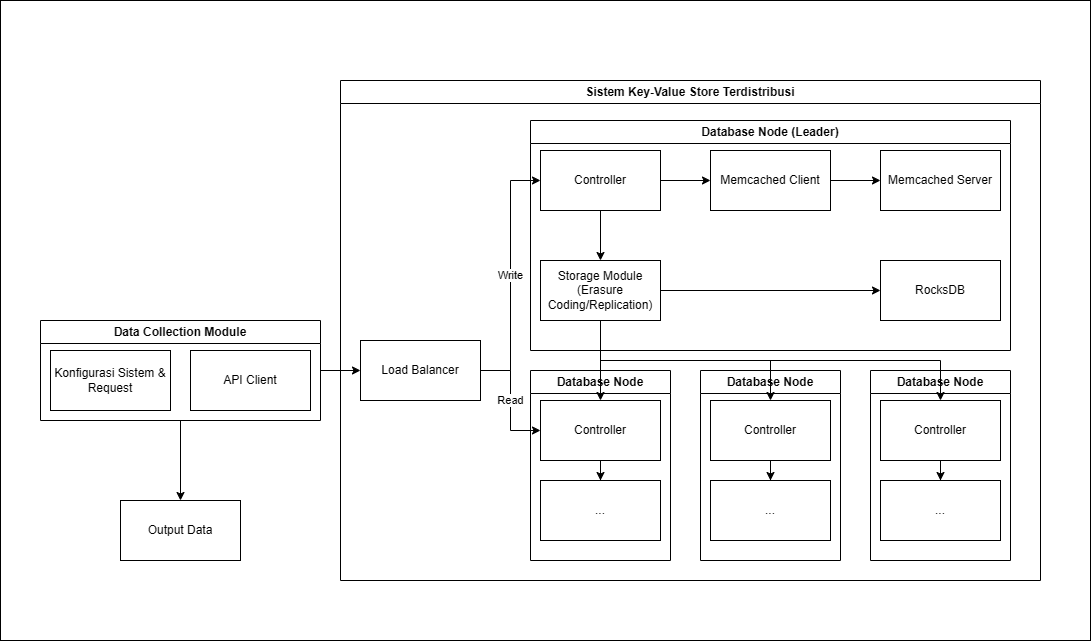
\includegraphics[width=0.95\textwidth]{resources/chapter-3/general-architecture.png}
    \caption{Struktur Komponen Logging dan Tracing}
    \label{fig:logging-tracing-structure}
\end{figure}
\subsubsection{Rancangan Detail Komponen Reporting}
\label{subsubsection:detail-reporting}

Komponen \textit{reporting} bertanggung jawab untuk menghasilkan laporan berdasarkan data yang telah dikumpulkan oleh komponen \textit{data collector}. Komponen ini akan memproses data dan menghasilkan visualisasi yang dapat digunakan untuk analisis lebih lanjut.

Ilustrasi struktur komponen \textit{reporting} dapat dilihat pada gambar \ref{fig:reporting-structure}.

% _TODO: Change image
\begin{figure}[ht]
    \centering
    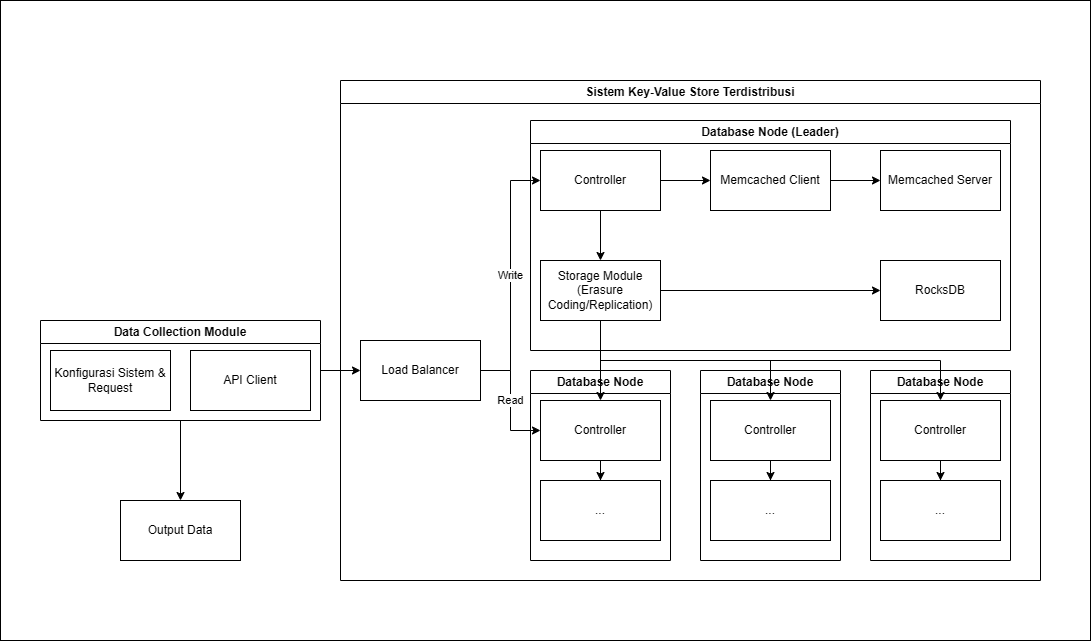
\includegraphics[width=0.95\textwidth]{resources/chapter-3/general-architecture.png}
    \caption{Struktur Komponen Reporting}
    \label{fig:reporting-structure}
\end{figure}
